\documentclass[border=10pt]{standalone}

\usepackage{tikz}
\usepackage{tikzsymbols}
\usetikzlibrary{calc,patterns,shapes.geometric}

\def\centerarc[#1](#2)(#3:#4:#5){\draw[#1] ($(#2)+({#5*cos(#3)},{#5*sin(#3)})$) arc (#3:#4:#5);}

\begin{document}
	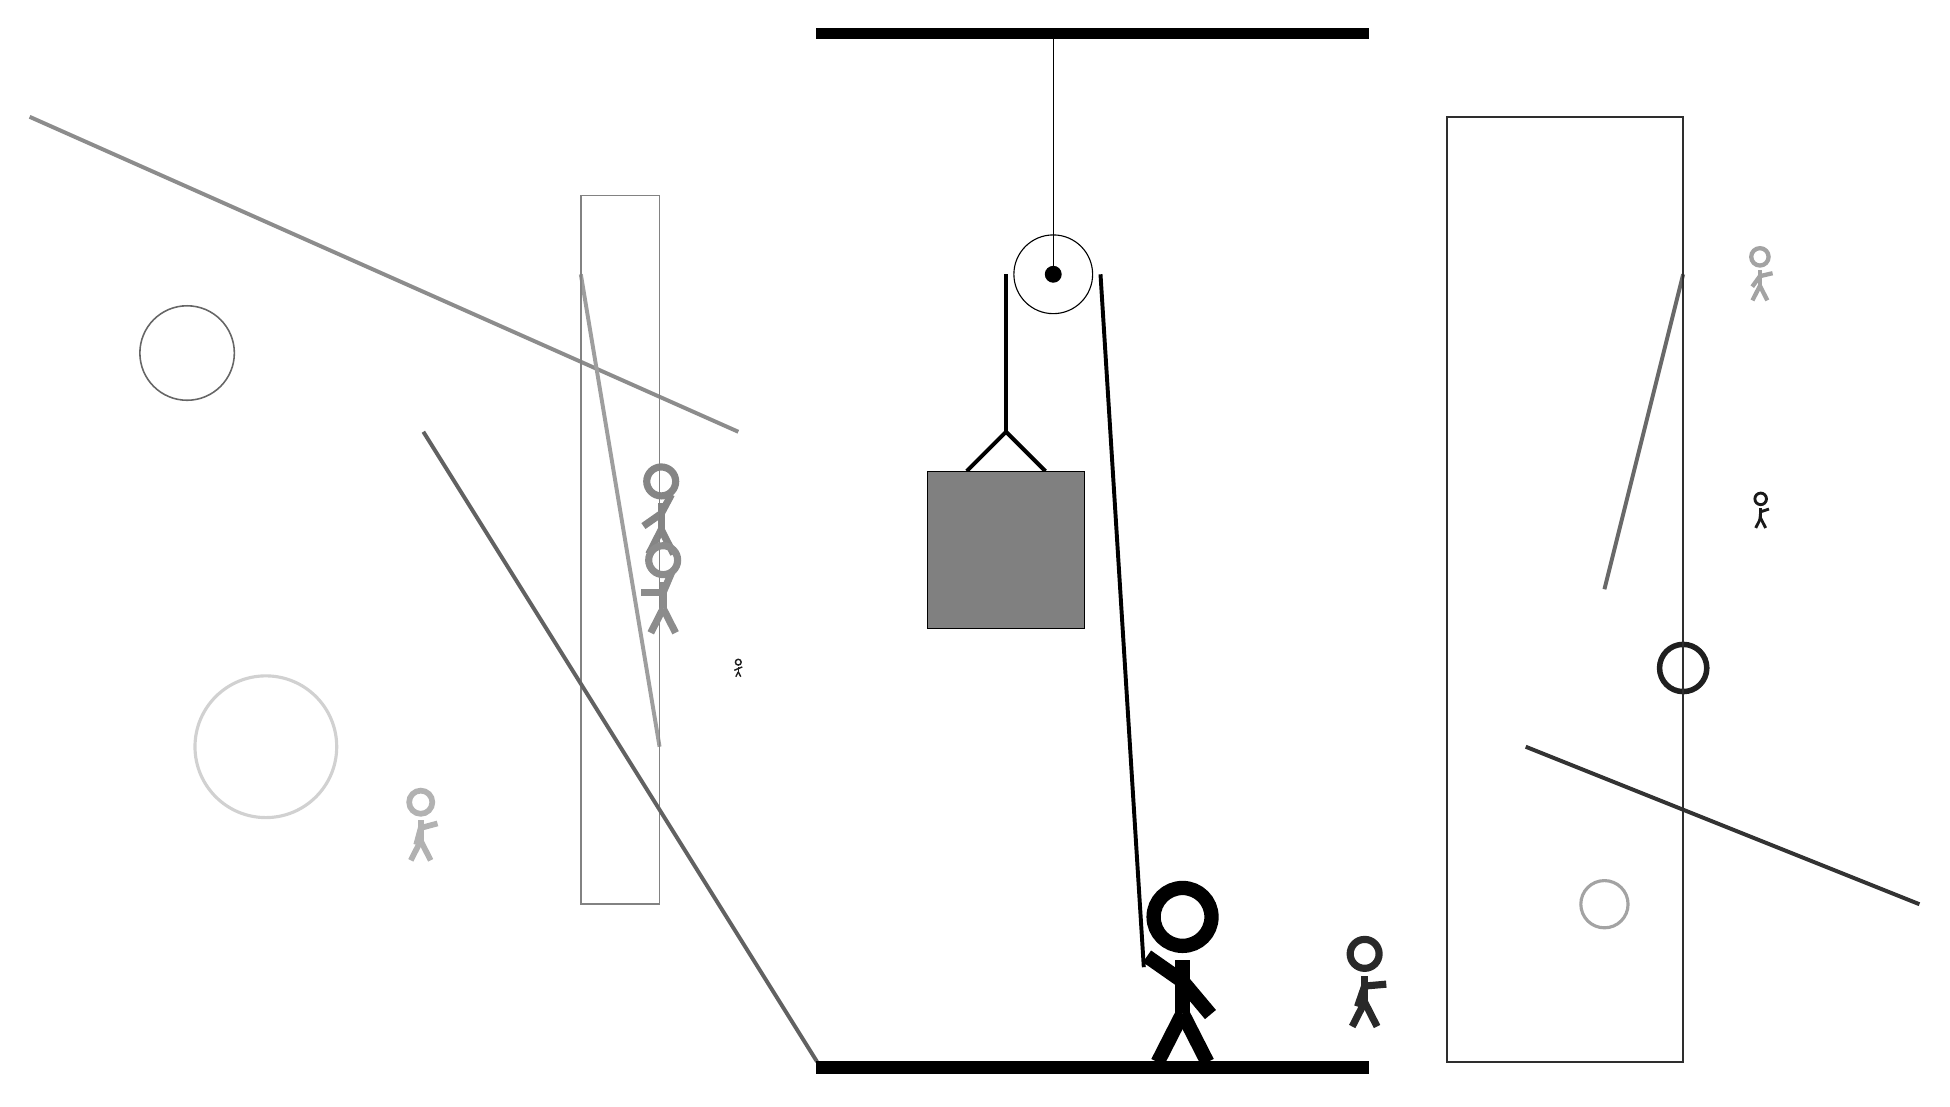
\begin{tikzpicture}
		%%%%% START %%%%%
		
		\draw[fill=black] (-2, 10) rectangle (5, 10.125);
		
		\draw (1, 7) circle (0.5);
		\draw[fill=black] (1, 7) circle (0.1);
		\draw (1, 10) -- (1, 7);
		
		\node[line width=0.4mm, color=black!84] at (5, -2) {\Strichmaxerl[5][71][5]};
		
		\draw[line width=0.5mm, color=black!45](-3, 5) -- (-12, 9);
		\draw [line width=0.4mm, color=black!36](8, -1) circle (0.3);
		\node[line width=0.5mm, color=black!48] at (-4, 4) {\Strichmaxerl[5][35][62]};
		\draw[line width=0.5mm, color=black!38](-4, 1) -- (-5, 7);
		\node[line width=0.7mm, color=black!36] at (10, 7) {\Strichmaxerl[3][54][13]};
		
		\draw[line width=0.5mm, color=black!80](7, 1) -- (12, -1);
		
		\draw[line width=0.5mm, color=black!59](9, 7) -- (8, 3);
		\draw[line width=0.2mm, color=black!49] (-4, 8) rectangle (-5, -1);
		\draw[line width=0.5mm, color=black!62](-2, -3) -- (-7, 5);
		\node[line width=0.3mm, color=black!30] at (-7, 0) {\Strichmaxerl[4][75][15]};
		
		\draw [line width=0.2mm, color=black!60](-10, 6) circle (0.6);
		\node[line width=0.7mm, color=black!45] at (-4, 3) {\Strichmaxerl[5][0][67]};
		\node[line width=0.2mm, color=black!88] at (-3, 2) {\Strichmaxerl[1][23][23]};
		\node[line width=0.2mm, color=black!90] at (10, 4) {\Strichmaxerl[2][84][18]};
		\draw [line width=0.7mm, color=black!88](9, 2) circle (0.3);
		\draw [line width=0.4mm, color=black!18](-9, 1) circle (0.9);
		\draw[line width=0.3mm, color=black!82] (6, -3) rectangle (9, 9);
		
		\draw[line width=0.5mm] (-0.1, 4.5) -- (0.4, 5.0) -- (0.9, 4.5);
		\draw[fill=black!50] (-0.6, 4.5) rectangle (1.4, 2.5);
		
		\draw[line width=0.5mm] (0.4, 7) -- (0.4, 5.0);
		\centerarc[line width=0.5mm](1, 7)(0:180:0.6);
		\draw[line width=0.5mm](1.6, 7) -- (2.15, -1.8);
		
		\node at (2.6, -1.9) {\Strichmaxerl[10][-35][-50]};
		
		\draw[fill=black] (-2, -3) rectangle (5, -3.15);
		
		%%%%% END %%%%%
	\end{tikzpicture}
\end{document}